\documentclass[english]{article}
%\documentclass[12pt,chapterheads]{ucsd}

%\usepackage[nodayofweek]{datetime}

%\usepackage[left=1.5in,right=1.5in,top=1.5in,bottom=1.5in]{geometry}
\usepackage[paper=letterpaper]{geometry}
\usepackage[affil-it]{authblk}

%\title{\textbf{Title} \\subtitle}
%\author{Zhao Lyu}
%\date{2018-01-15}%change \today

%\bibliographystyle{apa}
\usepackage{amsmath, mathtools, amsfonts,amssymb,flexisym,enumitem,grffile,graphicx,tikz,subcaption,titling}
\usepackage{tikz}
\usetikzlibrary{intersections,positioning,calc}
\usepackage{tkz-euclide}
\usetkzobj{all}
%\usepackage{wrapfig,blindtext,babel,calc}
%\usetikzlibrary{intersections,calc}
\usepackage{setspace}
\usepackage{url}
\setlist[enumerate]{itemsep=0mm}
%\graphicspath{{/home/user/Project199/Figures}}

\usepackage{amsthm}
\newtheorem*{definition*}{Definition}
\newtheorem{definition}{Definition}
\newtheorem{theorem}{Theorem}
\newtheorem*{theorem*}{Theorem}
\newtheorem*{lemma*}{Lemma}
\newtheorem{lemma}{Lemma}
\newtheorem*{claim*}{Claim}
\newtheorem{claim}{Claim}

\newcommand{\vol}{\operatorname{vol}}
\newcommand{\diam}{\operatorname{diam}}


\begin{document}
  % TODO : put the following lines ....

  \doublespacing %use setspace package
  \pagenumbering{gobble}
  %\maketitle{Refinement Strategy in 2 Dimension}
  \title{\textbf{Simplicial Mesh Refinement\\ in Computational Geometry}}
  \author{Zhao Lyu}
  \affil{Department of Mathematics, University of California, San Diego}
  \maketitle
  \singlespacing

  \newpage %separate title and contents
  %\pagenumbering{gobble}
  \tableofcontents
  \newpage
  \pagenumbering{arabic}

% ... up to here in a file, called frontmatter.tex, and \input it again.
  %\input{template}

  \section{Introduction}
  One question in computational geometry is how to represent complicated geometric shapes as a composition of more simple shapes. For example, an area can be expressed as a composition of triangles, and a volume can be written as a composition of tetrahedra. In this thesis, we discuss an important topic about such decompositions, namely the refinement of simplicial meshes.

One motivation for this topic is the numerical analysis of partial differential equations. While numerical methods simulate the behavior of a partial differential equation over some area, it is necessary  to represent the area on a computer first. This process is called triangulation, decomposing the area into simplices. Importantly, we sometimes may want to increase the resolution of this triangulation. To do so, algorithms which perform simplicial mesh refinement are crucial and worthy of attention. Besides its application in partial differential equations \cite{grosso1998hierarchical}, mesh refinement can also be applied in other fields, such as solving interpolation problems \cite{moore1992simplical}.

There are two main challenges in designing such algorithms. One is to maintain the stability of these simplices. In other words, unlimited to how many times a refinement is repeated, shapes of triangles should be bounded. That is, there should not exist any degenerating triangles, which refer to those with extremely small angles. One main reason why degenerating triangles should be avoided is that these triangles lead to ill-conditioned matrices in numerical methods for partial differential equations \cite{bank1989conditioning}. Another challenge is to  preserve the consistency of the triangulation. This means that two triangles either do not touch or only touch at a common edge or vertex, and the importance of this attribute is that an algorithm is expected to refine triangles consistently and successfully. In short, these two constraints make the development of algorithms for simplicial mesh refinement a challenging problem.

In this thesis, we discuss two applicable algorithms for mesh refinement in two dimensions. The first algorithm is called uniform refinement, one popular global refinement, of which the refinement is done all at once \cite{bank1983some,Bey1995,bey2000simplicial}. Though its easy application and obvious qualification for stability and consistency bring a popularity to this refinement strategy, it fails to provide some flexibility in refining simplicial meshes since uniform refinement is applied to whole simplices simultaneously. This is because uniform refinement forces to refine the entire mesh at once. However, many applications demand the flexibility to refine the mesh only locally. Thus, another algorithm, called the newest vertex bisection, is introduced to obtain such flexibility for local mesh refinement. However, newest vertex bisection is not perfect either. While newest vertex bisection of a single triangle preserves stability, preservation of consistency becomes complicated. In detail, the problem is that bisecting one triangle may depend on bisection of another. This leads to a chain reaction, which can be understood as a recursion using a stack and traversing back only when a base case is touched. Therefore, the difficulty is to determine how many triangles are part of this chain reaction, and under which conditions this chain reaction ends. In other words, it is not trivial whether the algorithm terminates and how long it lasts. 

In conclusion, this thesis will introduce uniform refinement and newest vertex bisection in two dimensions for computational geometry, and prove their stability and consistency in application, and further discuss their potential limits, possible solutions and their application in three dimensions and difficulties.


  %\newpage

  \section{Basic Definition}
    In this section, we introduce basic notions which we will use to present mesh refinement, and prove stability of uniform mesh refinement and bisection in later sections.
    We first recall definition of linear transformation and translation, and further introduce affine transformation.

       \subsection{Translation, Linear Transformation and Affine Transformation(pf for stability)}
      
      We define several classes of transformations that we use frequently.
      %sets\\
      linear, translation, affine transformation\\
      
      \begin{definition*}
        %$\textbf{Translation}$\\
         Let $\textbf{v}$ be a fixed vector, a $\textbf{Translation}$ ${T}_v$ on a figure applies as ${T}_v (\textbf{p}) = \textbf{p} + \textbf{v}$, for a vector $\textbf{p}$ in the figure which we translate.
      \end{definition*}
      A $\textit{translation}$ moves every point of a figure or space by the same distance in the same direction. A translation ${T}$ can be represented by an addition of a constant vector to every point.\\


      \begin{definition*}
      %\paragraph{Linear transformation}
      Let ${V}$ and ${W}$ be vector spaces over the same field $\textbf{K}$. We say a function $\mathit{f}: {V} \rightarrow {W}$ is $\textbf{linear transformation}$ if the following satisfied:\\
      \begin{align*}
      \mathit{f}(\textbf{u} + \textbf{v}) &= \mathit{f}(\textbf{u}) + \mathit{f}(\textbf{v}) \qquad \forall \textbf{u}, \textbf{v} \in{V},\\
      \mathit{f}(c\textbf{u}) &= c\mathit{f}(\textbf{u}), \qquad \forall \textbf{u} \in{V}, ~c\in\textbf{K}.
      \end{align*}
      \end{definition*}
      In other words, a linear transformation is a mapping between two vector spaces which preserves the operations of addition and scalar multiplication. Moreover, if ${V}$ and ${W}$ are finite dimentional, we can represent the linear transformation ${f}$ by a matrix ${M}$. For example, if ${M}$ is an ${m} \times {n}$ matrix, then ${f}$ is a linear transformation from $\mathbf{R}^n$ to $\mathbf{R}^m$. \\


      \begin{definition*}
      %\paragraph{Affine Transformation}
      An $\textbf{affine transformation}$ from $\mathbb{R}^n$ to $\mathbb{R}^n$ is of the form\\
      \begin{equation*}
      {F}(x) = {Ax} + {v}, \qquad {x}\in\mathbb{R}^n,
      \end{equation*}
      where ${A}$ is a linear transformation $\in\mathbb{R}^{n\times n}$, and  ${v}$ is a translation vector in $\mathbb{R}^n$\\
      \end{definition*}
      Affine transformation preserves points, lines and planes, but need not preserve point zero in a linear space in contrast to linear transformtion. So we see that translation and linear transformation is affine, but the opposite is not true.\\
      \indent
      The inverse mapping $F^{-1} = {x} \mapsto {A}^{-1}({x} - {v})$ is also an affine transformation. Clearly, we see that an affine transformation ${F}$ is invertible if and only if ${A}$ is invertible by the way we defined ${F}^{-1}$. Affine transformation helps carry results from one simplex to another simplex in our discussion, and more details are covered after introducing ${Simplices}$ and ${Triangulations}$ in the next section.
        \subsection{Simplices}
    \noindent
    \begin{definition*}
    A $\textbf{k-simplex T}$ $\in{R}^n$ is a ${k-}$dimensional convex hull of ${k}$ + 1 vertices ${x}_0, \cdots, {x}_k \in \mathbb{R}^n$, which are affinely independent.\\
    \begin{equation*}
    \begin{split}
    {T} & = [{x}_0, \cdots, {x}_k ]\\
    & := \left\{{x} = \sum\limits_{i=0}^k \lambda_i {x}_i \Bigm| \sum\limits_{i=0}^k \lambda_i = 1 ~and~ 0 \leqslant \lambda_i \leqslant 1, 0 \leqslant i \leqslant k \right\}\\
    & := \left\{\lambda_0{x}_0 + \cdots + \lambda_k{x}_k \Bigm| \sum\limits_{i=0}^k \lambda_i = 1 ~and~ 0 \leqslant \lambda_i \leqslant 1, 0 \leqslant i \leqslant k \right\}.
    \end{split}
    \end{equation*}
    \end{definition*}
    If ${k} = n$, we can call ${k-simplex}$ without addressing the dimension. 2-simplices are also called ${triangle}$, and 3-simplices are called ${tetrahedra}$.

    \begin{definition*}
    %\paragraph{Subsimplices}
    An  ${l-}$simplex ${S} = [{y}_0, \cdots, {y}_l]$ is called an $\textbf{l-subsimplex}$ of ${k-}$simplex ${T} = [{x}_0, \cdots, {x}_k]$, if indices $0 \leqslant {i}_0 \leqslant \cdots\leqslant{i}_l \leqslant k$ with ${y}_i = {x}_i$, for $0 \leqslant l \leqslant k \leqslant n$.
    \end{definition*}
    Since there are $k+1$ vertices in ${k-}$simplex ${T}$, and $l+1$ vertices in ${l-}$subsimplex ${S}$, the number of ${l-}$subsimplex of ${k-}$simplex is $\binom{k+1}{l+1}$.


    %\paragraph{Simplices Equality}
    Consider simplices ${T} = [{x}_0, \cdots, {x}_k]$ and $\text{T\textprime} = [{y}_0, \cdots, {y}_k]$. We say these two simplices ${T}$ and ${T\textprime}$ are equal, i.e. ${T} = {T\textprime}$, if ${x}_i = {y}_i$ for $0 \leqslant i \leqslant k$. Note that the vertex ordering of simplex is fixed, so if two simplices ${T}$ and ${T\textprime}$ denote the same set but with different vertex ordering, they are not equal; instead, we say that ${T}$ coincides with ${T\textprime}$, i.e. ${T} \cong {T\textprime}$.

    \paragraph{Simplex under Affine Transformation}\mbox{}\\
    Instead of taking a single variable $x\in\mathbb{R}^n$ for affine transformation, we can take a subset S $\subset \mathbb{R}^n$, which contains $x\in\mathbb{R}^n$. Then the transformed set $S\textprime$ is
    \begin{equation*}
    S\textprime= {F}(x) = \left\{{F}(x) ~|~ x\in S \right\}.
    \end{equation*}
    Similarly, if we regard a k-dimensional simplex ${T} = [{x_0, \cdots, x_k}]$ as a subset $\in\mathbb{R}^n$, then the image of ${T}$ under affine transformation, denoted by $T\textprime$, is defined as
    \begin{equation*}
    \begin{split}
    {T}\textprime & = {F}({T}) = \left\{{F}(x_0), \cdots , {F}(x_k)\right\}.
    \end{split}
    \end{equation*}
    We can see that ${T}\textprime$ is still a k-dimensional simplex. Furthermore, we can define ${F}({T}) = {AT} + {v}$, where $T$ is k-dimensional simplex $\in\mathbb{R}^n$. We might be curious about the relationship between simplices ${T}$ and ${T}\textprime$. Since vertices of a simplex are in a specific given order, so different vertex ordering leads to different simplices. Therefore, there exists an unique affine transformation such that ${T} = {T}\textprime$. Another important property of simplices is congruence.

    \begin{definition*}
    Two simplices T, T' are defined to be congruent if they can be obtained from each other by rotation, mirroring, scaling, and translation, i.e. if there exists a scaling factor c $\in\mathbb{R}^{+}$, a translation vector $v\in\mathbb{R}^n$, and an orthogonal matrix $Q\in\mathbb{R}^{n\times n}$ such that
    \begin{equation*}
    T' = v + cQT
    \end{equation*}
    \end{definition*}
    \noindent
    When the two simplices $T, T'$ have same vertices but with different vertex ordering, we can translate it as $T' = F(T)$. Based on how we define the affine transformation, it's not hard to see that ${T} \cong {T}\textprime$. Then we say that ${T}$ and ${T}\textprime$ are in a same congruent class.
    \subsection{Shape Regularity Measure}\mbox{}\\
    $\textit{Shape measure}$ offers an objective mathematical measure on the overall quality of an Finite Element mesh, and this is helpful to explore the simplex regularity and to improve the quality of shapes of the elements. Different definitions are used for shape measure to present the quality of simplex, and we simply introduce the $\textit{geometric shape measure} ~\mu({T})$ of simplex ${T}$,  the one we use in this paper.

    \paragraph{Simplex Diameter and Volume}\mbox{}\\
    Let ${T} \in\mathbb{R}^n$ be a k-simplex where $k \leqslant n$, with vertices ${x}_0, \cdots, {x}_k \in\mathbb{R}^n$. We let diam$({T})^k$ denote the diameter of ${T}$, and we define
    \begin{equation*}
    %\operator???
    \operatorname{diam}({T})^k = \max \| x_i - x_j \|, \qquad 0\leqslant i\leqslant j\leqslant k.
    \end{equation*}
    In other words, diam$({T})^k$ is the longest distance between two vertices of ${T}$, which is equivalent to the length of the longest edge of ${T}$. If ${T}$ is a single vertex, then diam$({T}) = 0$.\\

    \noindent
    Let vol$^k$(${T}$) denote k-dimensional volume of ${T}$. We have
    \begin{equation*}
    \operatorname{vol^k} ({T}) = \frac{1}{k!}\cdot|\det(x_1-x_0, x_2-x_0,\cdots, x_k-x_0)|
    \end{equation*}
    \noindent
    If k = 0, then ${T}$ is a 0-dimensional simplex, i.e., a vertex. Then clearly, diam(${T}$) = 0, and vol$^0 ({T})$ = 1, the vol$^0$ of a single vertex is one.

    
    \paragraph{Shape Measure}\mbox{}\\
    Simplex diameter and volume are important to introduce shape measures. Here we define the {geometric shape measure} $\mu({{T}})$ of a simplex ${T}$ by
    \begin{equation*}
    \mu({{T}}) = \frac{\operatorname{diam}({T})^k}{\operatorname{vol^k}({T})}, \quad\operatorname{vol^k(T) \neq 0}
    \end{equation*}
    If vol$^k(T)$ = 0, then we define $\mu({{T}}) = \infty$.\\
    
    To understand this definition, we can translate $\mu({{T}})$ as a measurement of how different the two variables, i.e. diam$({T})^k$ and vol$^k({T})$, are. For example, for a 3-dimensional simplex, i.e. a triangle, shape measure helps measure how narrow the triangle is. In other words, it measures how small the smallest angle of the triangle is. 

    \paragraph{Stability of a Simplex}\mbox{}\\
    The reason why we need shape measure is to help understanding whether a simplex $T$ is non-degenerate, and to quantify how degenerate or non-degenerate. Let $T$ be a k-dimensional simplex in $\mathbb{R}^n$. We say that a simplex $T$ is degenerate if and only if $\mu({T}) = \infty$, i.e. vol$_k(T) = 0$ approximating to 0.

    
    %???
    \begin{tikzpicture}
    \draw (0,0) -- (3,2) -- (5,0)-- (0,0);
    \draw (7,0) -- (10,1) -- (12,0)-- (7,0);
    %\path (1,1) coordinate (A) (2.5, 2.5) coordinate (B) (3, 1) coordinate (C)
    %\draw (A) -- (B) -- (C) -- cycle
    \end{tikzpicture}

    Observing two pictures above, we actually want the interior angles of the simple $T$, i.e. traingles in this example, to be uniformly bounded from zero. Thus vol$_2(T)$ will never go to 0.
    While cutting a simplex into smaller pieces, we want to keep those pieces uniformly bounded and avoid degenrate simplices. \\

    \begin{lemma*}
    If $T, T'$ are simplices that are congruent to each other, then $\mu(T) = \mu(T')$.
    \end{lemma*}
    \begin{proof}\mbox{}\\
    Since $T$ is congruent to $T'$, by definition, we have $T' = v + cQT$, where $c$ is scaling factor, $v$ is a translation vector and $Q$ is an orthogonal matrix. In fact, we will show that scaling, translation, roation or mirroring does not influence the shape measure of a simplex. 
    Suppose $diam(T)^k = ||x_i - x_j ||$, and $vol^k(T) = \frac{1}{k!}\cdot|\det(x_1-x_0, x_2-x_0,\cdots, x_k-x_0)|$.
    
    To be specific, when scaling a simplex $T$ by a non zero factor $c$ to obtain $T'$, we have 
    \begin{align*}
     vol^k(T') &= \frac{1}{k!}\cdot|\det(cx_1-cx_0, cx_2-cx_0,\cdots, cx_k-cx_0)| \\
               &= \frac{c^k}{k!}\cdot|\det(x_1-x_0, x_2-x_0,\cdots, x_k-x_0)| = c\cdot vol^k(T).
    \end{align*}
    Since it scales over all vertices, $diam(T')^k = c^k\cdot diam(T)^k$. Therefore, we see
    \begin{align*}
    \mu(T') = \frac{diam(T')^k}{vol^k(T')} = \frac{c^k\cdot diam(T)^k}{c^k\cdot vol^k(T)} = \frac{diam(T)^k}{vol^k(T)} = \mu(T)
    \end{align*}

    Moreover, translation over simplex $T$ by a nonsingular vector $v$ to obatin $T'$ will not influence the shape measure as well. In detail, we have
    \begin{align*}
    diam(T')^k &= ||(x_i + v) - (x_j + v)|| \\ 
               &= ||x_i - x_j|| = diam(T)^k \\
    vol^k(T') &= \frac{1}{k!}\cdot|\det((x_1+v) - (x_0+v), (x_2+v)-(x_0+v),\cdots,(x_k+v)-(x_0+v))|\\
              &= \frac{1}{k!}\cdot|\det(x_1-x_0, x_2-x_0,\cdots, x_k-x_0)| = vol^k(T)\\
    \mu(T') &= \frac{diam(T')^k}{vol^k(T')} = \frac{diam(T)^k}{vol^k(T)} = \mu(T)
    \end{align*}

    Consider rotating and mirroring $T$ by an orthogonal matrix $Q$ to obtain $T'$. Since $Q$ is an orthogonal matrix, $Q^T = Q^{-1}$. Therefore, we have
    \begin{align*}
    diam(T')^k &= ||Qx_i - Qx_j||\\
               &= ||x_i - x_j|| = diam(T)^k&&\\
    vol^k(T') = vol^k(Q\cdot T) &= \frac{1}{k!}\cdot |\det(Q(x_1-x_0), Q(x_2-x_0),\cdots, Q(x_k-x_0)|\\
                                &= \frac{1}{k!}\cdot|det(Q)|\cdot|\det(x_1-x_0, x_2-x_0, \cdots, x_k-x_0)|\\
                                &= \frac{1}{k!}\cdot|-1|\cdot|\det(x_1-x_0, x_2-x_0, \cdots, x_k-x_0)|\\
                                &= \frac{1}{k!}\cdot|\det(x_1-x_0, x_2-x_0, \cdots, x_k-x_0)| = vol^k(T)\\
    \text{Therefore, we have } \mu(T') &= \frac{diam(T')^k}{vol^k(T')}\\
    &= \frac{diam(T)^k}{vol^k(T)} = \mu(T)
    \end{align*}
    Now we see that the shape measure is independent of scaling, translation, rotation or mirroring. Thus a simplex $T'$ which is obtained by these motions shares a same shape measure with $T$.
    
    [ORIGINAL: ]
    First, we show that volumes of k-simplices $T$ and $T'$ are the same, i.e. vol$^k (T)$ = vol$^k (T')$. By definition of congruence, we can see one difference between equality and congruence of two simplices is that congruence is independent of vertex ordering. Recall the definition of simplex volume. \(vol^k(T) = \displaystyle \frac{1}{k!}\cdot|det(x_1-x_0, x_2-x_0,\cdots, x_k-x_0)|\). Clearly, permutation of vertex $x_i$, where $0 \leq i \leq k$, will not influence the absolute value of the determinant. Both dividing by k!, we have vol$^k (T)$ = vol$^k (T')$.\\
    Moreover, by definition of congruence above, we can obatin $T'$ by applying rotation, mirroring, scaling, and translation over $T$. Thus, diam$(T')^k$, the longest distance between two vertices of $T'$, is equal to the longest distance between two vertices of $T$, diam$(T)^k$. Therefore, we have $\mu(T) = \frac{diam(T)^k}{vol^k(T)} = \frac{diam(T')^k}{vol^k(T')} = \mu(T')$.
    \end{proof}
    % !TEX root = Prokect199.tex
\subsection{Simplicial Complex}
    \begin{definition}
    A $\emph{simplicial complex} ~~\mathcal T$ in $\mathbb{R}^n$ is a finite set of simplices in $\mathbb{R}^n$ that satisfies the following conditions:
    \begin{enumerate}[label =\arabic*.]
      \item Any subsimplex of a simplex from $\mathcal{T}$ is also in $\mathcal{T}$.
      \item The intersection of any two simplices ${T}_1, {T}_2 \in \mathcal{T}$ is a face of both ${T}_1$ and  ${T}_2$.
    \end{enumerate}
    \begin{figure}[b]
    \centering
    \captionsetup{justification=centering}
    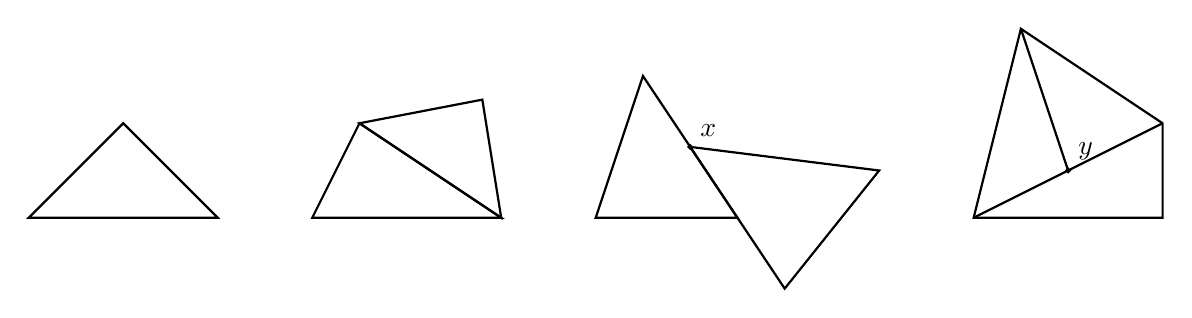
\begin{tikzpicture}[scale = 0.6]
    \coordinate (x) at (-6,0);
    \coordinate (y) at (-2,0);
    \coordinate (z) at (-4,2);
    \draw[thick] (x) -- (y) -- (z) -- cycle;

    \coordinate (a) at (0,0);
    \coordinate (b) at (4,0);
    \coordinate (c) at (1,2);
    \coordinate (d) at (3.6,2.5);
    \draw[thick] (a) -- (b) -- (c) -- cycle;
    \draw[thick] (d) -- (b) -- (c) -- cycle;

    \coordinate (a') at (6,0);
    \coordinate (b') at (9,0);
    \coordinate (c') at (7,3);
    \coordinate (d') at (12,1);
    \draw[thick] (a') -- (b') -- (c') -- cycle;
    \tkzDefMidPoint(b',c') \tkzGetPoint{bc}
    \fill[black!20, draw=black, thick] (bc) circle (1pt) node[black, above right] {$x$};
    \coordinate (e') at ($(bc)!2!0:(b')$);
    \draw[thick] (bc) -- (d') -- (e') -- cycle;
    
    \coordinate (q) at (14,0);
    \coordinate (w) at (18,0);
    \coordinate (e) at (15,4);
    \coordinate (r) at (18,2);
    \tkzDefMidPoint(q,r) \tkzGetPoint{mid}
    \draw[thick] (q) -- (w) -- (r) -- (e) -- cycle;
    \draw[thick] (q) -- (r);
    \draw[thick] (e) -- (mid);
    \fill[black!20, draw=black, thick] (mid) circle (1pt) node[black, above right] {$y$};

    \end{tikzpicture}
    %\includegraphics[width=60mm]{SimplicialComplex}
    \caption{Simplicial complex(left); Not simplicial complex(right)\\Two simplices in Figure\ref{Fig2} on the right are not simplicial complex because their intersection $x$ and $y$ are not shared. We call such nodes like $x$ and $y$ hanging node}%cite???
    \label{Fig2}
    \end{figure}
    \end{definition}
    In other words, the first condition asks $\mathcal{T}$ to be closed under taking subsimplices, and the second condition asks that the intersection of any two simplices is either a common subsimplex or empty because the empty set is a face of every simplex. Examples in 2D are shown in Figure \ref{Fig2}. 
    %Notice that two simplices in Figure\ref{Fig2} on the right are not simplicial complex because their intersection $x$ and $y$ are not shared. We call such nodes like $x$ and $y$ hanging node.

    Any subset ${T\textprime}\in{T}$ that is itself a simplicial complex is called a $\emph{subcomplex}$ of ${T}$. We say that a $\emph{simplicial $k$-complex}$ $\mathcal T$ is a simplicial complex where the largest dimension of any simplex in $\mathcal T$ is ${k}$. So a simplicial 2-complex must not contain tetrahedra or higher dimension simplices. The 0-complex of ${T}$ is called a $\textit{vertex set}$ of ${T}$. We can also think of a simplicial complex as a space with a triangulation, which is the division of a surface or a plane polygon into a set of 2-simplices. 

    \paragraph{Simplicial Complex under Affine Transformation---\textbf{DELETE???????}}\mbox{}\\
    Extending further from simplex under affine transformation, now we know that simplicial complex is just a finite set of simplices. Therefore, we can define the Transformed Simplicial Complex $F(\mathcal{T})$ as follows
    \begin{equation*}
    F(\mathcal{T}) := \{ \; F(T) \;\vert\; T \in \mathcal{T} \; \}
    \end{equation*}
    If $\mathcal{T}$ is consistent, then $F(\mathcal{T})$ is also consistent by inheriting this property from $\mathcal{T}$.

    \paragraph{Shape Measure of Simplicial Complex}\mbox{}\\
    Recall the definition of the shape measure of a simplex.
    Now consider a simplicial complex $\mathcal{T}$, we define the geometric shape measure $\mu(\mathcal{T})$ as follows,
    \begin{equation*}
    \mu(\mathcal{T}) = \max_{T \in \mathcal{T}} \mu(T)
    \end{equation*}
    By definition, we see that the shape measure of a simplicial complex $\mathcal{T}$ is the supremum of the set of shape measures of all simplices $T\in\mathcal{T}$. If the largest shape measure of a simplex in this simplicial complex is bounded, then none of the simplices in $\mathcal{T}$ are degenerate. %In other words, if simplex $T_0 \in\mathcal{T}$ is non-degenerate, then the simplicial complex $\mathcal{T}$ non-degenerate.
    %[Correct?? Pf needed???]


  \section{Refinement Strategies in General}
    Suppose that a domain is divided into simplices. Mesh refinement is a procedure of mesh modification in which we divide these simplices into smaller simplices. This process can be applied recursively. Let us first introduce triangulation to help understand refinement on a simplex. Generally speaking, we can think triangulation as a subdivision of a plane into triangles. The following definition is a more formal way to take when extending to a higher dimension.
    \begin{definition}
    A triangulation of $\mathbb R^n$ is subdivision into n-dimensional simplices such that intersection of any two simplices is either empty or sharing a common face, and any face of a simplex is in the triangulation.
    \end{definition}
    Indeed, we say that this triangulation is consistent as it is not simply subdividing of a space. Moreover, the triangulation defined here can be treated equivalently as simplicial complex as it is a finite set of simplices satisfying
    \begin{itemize}
        \item[1.] Any face of a simplex from a triangulation is also in the triangulation
        \item[2.] The intersection of any two simplices $T_1, T_2 $ in a triangulation is a face of both $T_1$ and  $T_2$ or empty
    \end{itemize}
    %(Denote triangulation same as simplicial complex $\mathcal{T}$)\\
    

    We can think a refinement of a simplex $T$ as a triangulation $\mathcal{T}$ which consists of smaller pieces of simplices of the same type of the simplex $T$. Now consider a refinement of a simplicial complex. Let $\mathcal{T}$ and $\mathcal{T'}$ be two different simplicial complexes covering a same domain $\Omega$. This means that the domain \(\Omega = \displaystyle \bigcup({T \vert T\in \mathcal{T}}) = \bigcup({T' \vert T\in \mathcal{T'}})\). We say that $\mathcal{T'}$ is a refinement of $\mathcal{T}$ if each simplex $T\in\mathcal{T}$ is in $\mathcal{T'}$ or the triangulation of $T$ is in $\mathcal{T'}$.

    As mentioned before, we may recursively apply a refinement strategy to help simplify some problems. By recursively taking refinement process from $\mathcal{T}_0$, we have a hierarchy triangulation $\mathcal{T}_k, k\in\mathbb{N}$, where $\mathcal{T}_k$ is a refinement of $\mathcal{T}_{k-1}$. 
    \begin{definition}
    Let $\mathcal{T}_0$ be the initial simplicial complex in $\mathbb{R}^n$ where it starts from, then we define the hierarchy triangulation $\mathcal{T}_k$ as follows
    \begin{equation*}
    \mathcal{T}_k := \bigcup\{refinement~of~simplex~T ~\vert ~T\in\mathcal{T}_{k-1}\}, \quad k\in\mathbb{N}
    \end{equation*}
    \end{definition}

    \subsection{Consistency of Refinement}
    We want the triangulation always to be consistent after applying a refinement. This feature is proved in section 2.4 that if either 1) any face of a simplex from this triangulation $\mathcal{T}$ is also in $\mathcal{T}$, or 2) the intersection of any two simplices in a face of both simplices.

    \subsection{Stability of Refinement}
    Besides consistency, we also want all simplices in a triangulation resulted from a refinement strategy non-degenerating so that we can apply the refinement strategy recursively to have nicely shaped triangulation in the end.
    
    \begin{definition}
    We say a refinement strategy is $\textbf{stable}$ if there exists a constant $C >$ 0 such that $\mu(T)< C$ for all simplices $T$.
    \end{definition}
    
    \begin{theorem*}
    If the number of congruence classes, obtained by applying the refinement of a non-degenerate simplex $T$ initially, is finite, then the refinement strategy is stable.
    \end{theorem*}
    \begin{proof}
    %Idea:\\
    %1. $T_0$ is non-degenerate, then $\mathcal{T_0}$ is non-degenerate.\\
    
    We claim that
    a refinement strategy over initial simplicial complex $T_0$ produces only non-degenerate simplices $T$.
    
    We prove this claim by induction.
    Clearly, the base case is true since it is given that all simplices $T$ in $\mathcal{T}$ are non-degenerate. For induction, suppose simplices in simplicial complex $\mathcal{T}_k$ is non-degenerate. That is, there exists $C > 0$ such that $\mu(T) < C, ~\forall T \in\mathcal{T}_k$. Apply the refinement strategy on $\mathcal{T}_k$, and then we obtain $\mathcal{T}_{k+1} = \bigcup\{refinement~of~simplex~T ~\vert ~T\in\mathcal{T}_{k}\}, \quad k\in\mathbb{N}$. 
    %[connection???: f simplex $T_0 \in\mathcal{T}$ is non-degenerate, then simplicial complex $\mathcal{T}$ non-degenerate.]
    
    Next, we show the following fact.
    If the number of congruence classes is finite, then the number of shape measure is finite, and there exists a common bound $C > 0$ such that $C \geq \mu(\mathcal{T})$.
    
    This can be seen as follows.
    We proved that simplices in same congruence classes share the same shape measure. If we have a finite number of congruence classes, clearly we have a finite number of shape measures. When all simplices are non-degenerate, we always have an upper bound for their shape measure $\mu(T)$. With the finite number of shape measures, we may set $C$ as the maximum of all upper bounds of shape measures. And therefore $C \geq \mu(\mathcal{T})$.
    
    Since $T_0$ is non-degenerate, $T_0$ is non-degenerate. Moreover, we know there exists a common bound $C$ for all shape measures since the number of congruence classes is finite. Therefore, we proved the stability.
    \end{proof}
    
    

  \section{Uniform Refinement}
  Intro para...
    [Al of uniform refinement in 2-d, show it's stable and consistent]
    \subsection{2D -[UPDATED]}
    One popular refinement strategy is $red/green$ refinement proposed by R. E. Bank. The red refinement here is regular refinement which divides a triangle into four congruent smaller triangles by connecting midpoints of its three edges. The green refinement is irregular refinement which connects the refined edge midpoint to its opposite corner.[PIC-NEED TO BE UPDATE]\\

    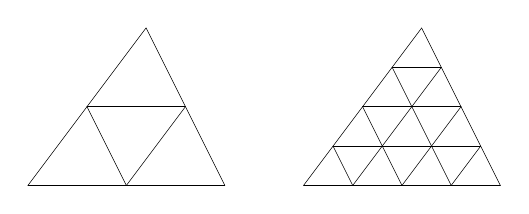
\begin{tikzpicture}
    \tkzDefPoint(0,0){A}
    \tkzDefPoint(1.5,2){B}
    \tkzDefPoint(2.5,0){C}
    \tkzDrawSegments(A,B B,C A,C)

    %\tkzLabelPoints[above,yshift=0pt](2)
    %\tkzLabelPoints[left,yshift=4pt](0)
    %\tkzLabelPoints[right,yshift=4pt](1)
    \tkzDefMidPoint(A,B) \tkzGetPoint{ab}
    \tkzDefLine[orthogonal=through ab](A,B)
    \tkzDefMidPoint(A,C) \tkzGetPoint{ac}
    \tkzDefLine[orthogonal=through ac](A,C)
    \tkzDefMidPoint(B,C) \tkzGetPoint{bc}
    \tkzDefLine[orthogonal=through bc](B,C)
    \tkzDrawSegment(ab,ac)
    \tkzDrawSegment(ab,bc)
    \tkzDrawSegment(ac,bc)

    \tkzDefPoint(3.5,0){A'}
    \tkzDefPoint(5,2){B'}
    \tkzDefPoint(6,0){C'}
    \tkzDrawSegments(A',B' B',C' A',C')
    \tkzDefMidPoint(A',B') \tkzGetPoint{ab'}
    \tkzDefLine[orthogonal=through ab'](A',B')
    \tkzDefMidPoint(A',C') \tkzGetPoint{ac'}
    \tkzDefLine[orthogonal=through ac'](A',C')
    \tkzDefMidPoint(B',C') \tkzGetPoint{bc'}
    \tkzDefLine[orthogonal=through bc'](B',C')
    \tkzDrawSegment(ab',ac')
    \tkzDrawSegment(ab',bc')
    \tkzDrawSegment(ac',bc')

    \tkzDefMidPoint(A',ab') \tkzGetPoint{aab}
    \tkzDefLine[orthogonal=through aab](A',ab')
    \tkzDefMidPoint(A',ac') \tkzGetPoint{aac}
    \tkzDefLine[orthogonal=through aac](A',ac')
    \tkzDefMidPoint(ac',ab') \tkzGetPoint{x}
    \tkzDefLine[orthogonal=through x](ac',ab')
    \tkzDrawSegment(aab,aac)
    \tkzDrawSegment(aab,x)
    \tkzDrawSegment(aac,x)

    \tkzDefMidPoint(B',ab') \tkzGetPoint{abb}
    \tkzDefLine[orthogonal=through abb](B',ab')
    \tkzDefMidPoint(B',bc') \tkzGetPoint{bbc}
    \tkzDefLine[orthogonal=through bbc](B',bc')
    \tkzDefMidPoint(bc',ab') \tkzGetPoint{y}
    \tkzDefLine[orthogonal=through y](bc',ab')
    \tkzDrawSegment(abb,bbc)
    \tkzDrawSegment(abb,y)
    \tkzDrawSegment(bbc,y)

    \tkzDefMidPoint(C',ac') \tkzGetPoint{acc}
    \tkzDefLine[orthogonal=through acc](C',ac')
    \tkzDefMidPoint(C',bc') \tkzGetPoint{bcc}
    \tkzDefLine[orthogonal=through bcc](C',bc')
    \tkzDefMidPoint(bc',ac') \tkzGetPoint{z}
    \tkzDefLine[orthogonal=through z](bc',ac')
    \tkzDrawSegment(acc,bcc)
    \tkzDrawSegment(acc,z)
    \tkzDrawSegment(bcc,z)

    \tkzDefMidPoint(ab',ac') \tkzGetPoint{l}
    \tkzDefLine[orthogonal=through l](ab',ac')
    \tkzDefMidPoint(ab',bc') \tkzGetPoint{m}
    \tkzDefLine[orthogonal=through m](ab',bc')
    \tkzDefMidPoint(ac',bc') \tkzGetPoint{r}
    \tkzDefLine[orthogonal=through r](ac',bc')
    \tkzDrawSegment(l,m)
    \tkzDrawSegment(l,r)
    \tkzDrawSegment(m,r)

    \end{tikzpicture}

    Let $T = [x^0, x^1, x^2]$ be the triangle to be refined, and denote $x^{ij}$ as the midpoint of the edge between $x^i$ and $x^j$.\\
    \textbf{Algorithm} Red refinement in 2D \{\\
    $T_1 := [x^0, x^{01}, x^{02}]; \qquad T_2 := [x^{01}, x^{1}, x^{12}];$\\
    $T_3 := [x^{02}, x^{12}, x^2]; \qquad T_4 := [x^{01}, x^{12}, x^{02}];$\\
    \}

    \begin{lemma*}
    Red refinement gives same congruence class in 2-dimension case.
    \end{lemma*}
    \begin{proof}\mbox{}\\

    \begin{tikzpicture}[scale=0.75]
    \tkzDefPoint(0,0){A}
    \tkzDefPoint(1.5,2){B}
    \tkzDefPoint(2.5,0){C}
    \tkzDrawSegments(A,B B,C A,C)

    \tkzLabelPoints[above,yshift=0pt](B)
    \tkzLabelPoints[left,yshift=4pt](A)
    \tkzLabelPoints[right,yshift=4pt](C)
    \tkzDefMidPoint(A,B) \tkzGetPoint{X}
    \tkzDefLine[orthogonal=through ab](A,B)
    \tkzDefMidPoint(A,C) \tkzGetPoint{Z}
    \tkzDefLine[orthogonal=through ac](A,C)
    \tkzDefMidPoint(B,C) \tkzGetPoint{Y}
    \tkzDefLine[orthogonal=through bc](B,C)
    \tkzDrawSegment(X,Z)
    \tkzDrawSegment(X,Y)
    \tkzDrawSegment(Z,Y)
    \tkzLabelPoints[above,xshift=-2mm](X)
    \tkzLabelPoints[above,xshift=2mm](Y)
    \tkzLabelPoints[below](Z)
    \end{tikzpicture}

    By red refinement, we have X, Y and Z as midpoints of edges AB, BC and AC. Thus, line XY parallel to line AC, i.e., $XY \parallel AC$, so $\angle{BXY} = \angle{XAZ}$. Similarily, since $XZ\parallel BC$, $\angle{XBY} = \angle{AXZ}$. Since X is the midpoint of line AB, then AX = BX. In short, we have 
    \begin{align*}
    \angle{BXY} &= \angle{XAZ}\\
    BX &= AX\\
    \angle{XBY} &= \angle{AXZ}
    \end{align*}
    Therefore, $\triangle{BXY} \cong \triangle{XAZ}$. Similarily, we can prove the four triangles are congruent to each other, i.e., $\triangle{BXY}\cong\triangle{XAZ}\cong\triangle{YZC} \cong\triangle{ZYX}$, so they are in a same congruent class, which is similar to the original triangle $\triangle{BAC}$.
    \end{proof}
    By lemma, we know that red refinement applied on a non degenerate simplex in 2 dimension gives one congruent class. Moreover, by Theorem in 3.1, we see that red refinement strategy is stable.
    [This lemma leads to stability]

    \begin{lemma*}
    Red refinement preserves consistency in 2-dimension case.
    \end{lemma*}
    \begin{proof}\mbox{}\\
    Question1: show they are all simplicial complex by definition?
    \end{proof}
    Subdividing a triangle by connecting its midpoint, we obtain four congruent simplices $T_1, T_2, T_3$ and $T_4$. The green refinement is applied on one refined edge on which we may confront with degenerate simplices. We will never touch and refine such simplices to avoid them from degenerating.

    
    Clearly, the red refinement strategy is stable since it produces a finite number of triangles congruenct to the original simplex. Meanwhile, we preserve consistency by bisecting triangles with one refined edge and never refine them any further. Therefore, we obtain stability and consistency through red and green refinement.

    \subsection{3D}

  \section{Newest Vertex Bisection}
        \subsection{Bisection Refinement in 2-dimension and its stability}
    Another popular refinement strategy is bisection. Basically, we cut a triangle by connecting one vertex, which we choose as the peak, with its opposite edge, which we call refinement edge. Generally, if we apply random bisection with no plan on a triangle, it is likely that we fail to preserve stability and consistency.

    Hence, one important part we need to consider is how to choose the peak for a triangle to preserve the stability and consistency, and one famous method was introduced as the $newest vertex$ bisection. In newest vertex bisection, we create the newest vertex at the middle of the refinement edge after applying the bisection refinement once, and then we regard the newest vertex as the peak for bisection over the resulting two smaller triangles.

    \begin{figure}[h!]
    \centering
      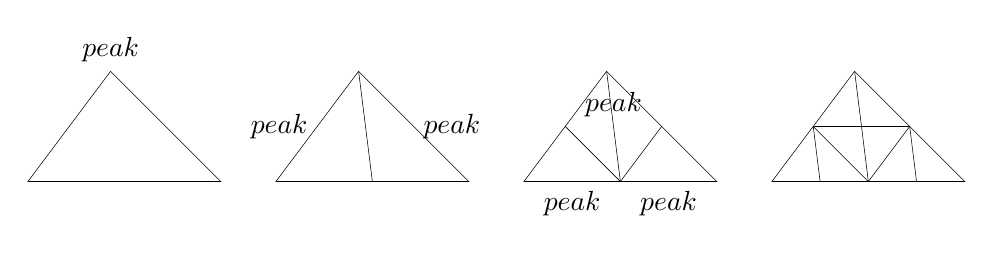
\begin{tikzpicture}[scale=0.7]
      \tkzDefPoint(-6.5,0){A''}
      \tkzDefPoint(-5,2){peak}
      \tkzDefPoint(-3,0){C''}
      \tkzDrawSegments(A'',peak peak,C'' A'',C'')
    %\tkzDrawSegments(A'',B'' B'',C'' A'',C'')
      \tkzLabelPoints[above,yshift=0pt](peak)
    %\tkzDefMidPoint(A'',C'') \tkzGetPoint{new vertex}
    %\tkzLabelPoints[below,yshift=0pt](new vertex)
    %\tkzDefLine[orthogonal=through ac](A,C)
    
    \tkzDefPoint(-2,0){A}
    \tkzDefPoint(-0.5,2){B}
    \tkzDefPoint(1.5,0){C}
    \tkzDrawSegments(A,B B,C A,C)
    \tkzDefMidPoint(A,B) \tkzGetPoint{peak}
    \tkzLabelPoints[left](peak)
    \tkzDefMidPoint(B,C) \tkzGetPoint{peak}
    \tkzLabelPoints[right](peak)
    \tkzDefMidPoint(A,C) \tkzGetPoint{ac}
    \tkzDefLine[orthogonal=through ac](A,C)
    \tkzDrawSegment(B,ac)


    \tkzDefPoint(2.5,0){A'}
    \tkzDefPoint(4,2){B'}
    \tkzDefPoint(6,0){C'}
    \tkzDrawSegments(A',B' B',C' A',C')
    \tkzDefMidPoint(A',B') \tkzGetPoint{ab'}
    \tkzDefLine[orthogonal=through ab'](A',B')
    \tkzDefMidPoint(A',C') \tkzGetPoint{ac'}
    \tkzDefLine[orthogonal=through ac'](A',C')
    \tkzDefMidPoint(B',C') \tkzGetPoint{bc'}
    \tkzDefLine[orthogonal=through bc'](B',C')
    \tkzDrawSegment(B',ac')
    \tkzDrawSegment(ac',ab')
    \tkzDrawSegment(ac',bc')
    \tkzDefMidPoint(B',ac') \tkzGetPoint{peak}
    \tkzLabelPoints[above,yshift=0pt](peak)
    \tkzDefMidPoint(A',ac') \tkzGetPoint{peak}
    \tkzLabelPoints[below](peak)
    \tkzDefMidPoint(C',ac') \tkzGetPoint{peak}    
    \tkzLabelPoints[below](peak)


    \tkzDefPoint(7,0){A'''}
    \tkzDefPoint(8.5,2){B'''}
    \tkzDefPoint(10.5,0){C'''}
    \tkzDrawSegments(A''',B''' B''',C''' A''',C''')
    \tkzDefMidPoint(A''',B''') \tkzGetPoint{ab''}
    \tkzDefLine[orthogonal=through ab''](A''',B''')
    \tkzDefMidPoint(A''',C''') \tkzGetPoint{ac''}
    \tkzDefLine[orthogonal=through ac''](A''',C''')
    \tkzDefMidPoint(B''',C''') \tkzGetPoint{bc''}
    \tkzDefLine[orthogonal=through bc''](B''',C''')
    \tkzDrawSegment(B''',ac'')
    \tkzDrawSegment(ac'',ab'')
    \tkzDrawSegment(ac'',bc'')
    \tkzDefMidPoint(B''',ac'') \tkzGetPoint{x}
    \tkzDefLine[orthogonal=through x](B''',ac'')
    \tkzDefMidPoint(A''',ac'') \tkzGetPoint{y}
    \tkzDefLine[orthogonal=through y](A''',ac'')
    \tkzDefMidPoint(C''',ac'') \tkzGetPoint{z}
    \tkzDefLine[orthogonal=through z](C''',ac'')
    \tkzDrawSegment(ab'',x)
    \tkzDrawSegment(bc'',x)
    \tkzDrawSegment(ab'',y)
    \tkzDrawSegment(bc'',z)
    \end{tikzpicture}
    \caption{Illustration of bisection refinement, starting with a single triangle}
    \label{Fig4}
    \end{figure}







%----------------------------------------------------------------------------------
    %\subsection{Stability of Newest Vertex Bisection}
    \begin{lemma*}
    Bisection refinement gives four congruence classes given one triangle.
    \end{lemma*}
    \begin{proof}
    \begin{figure}[h!]
    \centering
      \begin{tikzpicture}[scale=0.8]
      \tkzDefPoint(-9,0){A''}
      \tkzDefPoint(-7.5,2){B''}
      \tkzDefPoint(-5.5,0){C''}
      \tkzDrawSegments(A'',B'' B'',C'' A'',C'')
      \node (t) at (-7.5, 1) {{1}};

      \tkzDefPoint(-2,0){A}
      \tkzDefPoint(-0.5,2){B}
      \tkzDefPoint(1.5,0){C}
      \tkzDrawSegments(A,B B,C A,C)
      \tkzDefMidPoint(A,C) \tkzGetPoint{ac}
      \tkzDefLine[orthogonal=through ac](A,C)
      \tkzDrawSegment(B,ac)
      \node (t') at (-1, 0.5) {{2}};
      \node (t'') at (0.5, 0.5) {{3}};
      \end{tikzpicture}
    \caption{Stage 1: Original triangle(left); Stage 2: Applied the newest vertex bisection once(right)}
    \label{fig5: sub1}
    \end{figure}

    Observing Figure 5, we have a triangle at the beginning, say it's in congruency class 1. After applying the newest vertex bisection refinement once, we obtain two smaller pieces of triangles as in the second picture in Figure 5. Say one of them is in congruency class 2, and another one is in congruency class 3. Further applying the newest vertex bisection refinement, we have the figures below.

    \begin{figure}[h!]
    \centering
      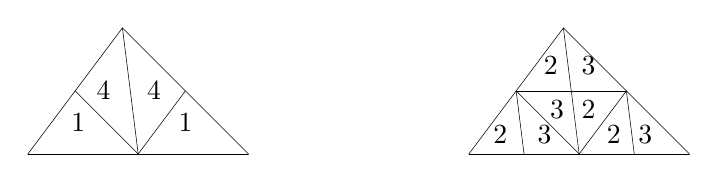
\begin{tikzpicture}[scale=0.8] 
      \tkzDefPoint(0,0){A'}
      \tkzDefPoint(1.5,2){B'}
      \tkzDefPoint(3.5,0){C'}
      \tkzDrawSegments(A',B' B',C' A',C')
      \tkzDefMidPoint(A',B') \tkzGetPoint{ab'}
      \tkzDefLine[orthogonal=through ab'](A',B')
      \tkzDefMidPoint(A',C') \tkzGetPoint{ac'}
      \tkzDefLine[orthogonal=through ac'](A',C')
      \tkzDefMidPoint(B',C') \tkzGetPoint{bc'}
      \tkzDefLine[orthogonal=through bc'](B',C')
      \tkzDrawSegment(B',ac')
      \tkzDrawSegment(ac',ab')
      \tkzDrawSegment(ac',bc')
      \node (t''') at (1.2, 1) {{4}};
      \node (t''') at (2, 1) {{4}};
      \node (t) at (0.8, 0.5) {{1}};
      \node (t) at (2.5, 0.5) {{1}};

      \tkzDefPoint(7,0){A'''}
      \tkzDefPoint(8.5,2){B'''}
      \tkzDefPoint(10.5,0){C'''}
      \tkzDrawSegments(A''',B''' B''',C''' A''',C''')
      \tkzDefMidPoint(A''',B''') \tkzGetPoint{ab''}
      \tkzDefLine[orthogonal=through ab''](A''',B''')
      \tkzDefMidPoint(A''',C''') \tkzGetPoint{ac''}
      \tkzDefLine[orthogonal=through ac''](A''',C''')
      \tkzDefMidPoint(B''',C''') \tkzGetPoint{bc''}
      \tkzDefLine[orthogonal=through bc''](B''',C''')
      \tkzDrawSegment(B''',ac'')
      \tkzDrawSegment(ac'',ab'')
      \tkzDrawSegment(ac'',bc'')
      \tkzDefMidPoint(B''',ac'') \tkzGetPoint{x}
      \tkzDefLine[orthogonal=through x](B''',ac'')
      \tkzDefMidPoint(A''',ac'') \tkzGetPoint{y}
      \tkzDefLine[orthogonal=through y](A''',ac'')
      \tkzDefMidPoint(C''',ac'') \tkzGetPoint{z}
      \tkzDefLine[orthogonal=through z](C''',ac'')
      \tkzDrawSegment(ab'',x)
      \tkzDrawSegment(bc'',x)
      \tkzDrawSegment(ab'',y)
      \tkzDrawSegment(bc'',z)
      \node (t') at (7.5, 0.3) {{2}};
      \node (t'') at (8.2, 0.3) {{3}};
      \node (t'') at (8.4, 0.7) {{3}};
      \node (t') at (8.3, 1.4) {{2}};
      \node (t'') at (8.9, 1.4) {{3}};
      \node (t') at (8.9, 0.7) {{2}};
      \node (t') at (9.3, 0.3) {{2}};
      \node (t'') at (9.8, 0.3) {{3}};
      \end{tikzpicture}
    \caption{Stage 3: Applied the newest vertex bisection twice(left); Stage 4: Applied the newest vertex bisection three times(right)}
    \label{fig5: sub2}
    \end{figure}

    \begin{claim}
    The left and right bottom triangles in Stage 3 are congruent to the original triangle in Stage 1, and they are in the congruency class 1. Moreover, the other two triangles left are congruent and in congruency class 4.
    \end{claim}
    %\begin{proof}\mbox{}\\
    \noindent
    Proof of Claim 1: \\
    Let A, B, C be the vertices of the triangle $T$ and let X, Y, Z be the midpoints of the edge AB, AC and BC. An application of the newest vertex bisection refinement produces the triangle $\triangle{AXY}, \triangle{XBY}, \triangle{ZBY}$ and $\triangle{YZC}$. Consider the Fig 8 (left).
    Since X, Y, Z be the midpoints of the edge AB, AC and BC, we have 
    \begin{align*}
     XY \parallel BC,
     \quad 
     ZY \parallel AB,
     \quad 
     AX = BX, 
     \quad 
     BZ = CZ, 
     \quad
     AY = CY
    \end{align*}
    Since $XY\parallel BC$, we have $\angle{AXY} = \angle{ABC}$ and $\angle{XYB} = \angle{ZBY}$. Similarly, since $ZY\parallel AB$, we have $\angle{YZC} = \angle{ABC}$ and $\angle{XBY} = \angle{ZYB}$. Thus 
    \begin{align*}
    \angle{XYB} = \angle{ZBY},
    \quad
    |BY| = |BY|,
    \quad
    \angle{XBY} &= \angle{ZYB}.
    \end{align*}
    Therefore, we have $\triangle{XBY} \cong \triangle{ZYB}$, and we mark them in the congruency class 4. This further gives us $|AX| = |BX| = |YZ|$, and $|ZC| = |BZ| = |XY|$.
    \begin{align*}
    |AX| = |YZ|,
    \quad
    \angle{AXY} = \angle{ABC} = {YZC},
    \quad
    |XY| = |ZC|.
    \end{align*}
    Therefore, we have $\triangle{AXY} \cong \triangle{YZC}$. It's clear that $\triangle{AXY}$ and $\triangle{YZC}$ are similar to $\triangle{ABC}$ as all their angles are the same. Thus, we finished the proof of claim 1.

    %\end{proof}%end proof of claim 1

    \begin{claim}
    Triangles with same number in Stage 4 in a same congruency class marked by the number.
    \end{claim}
    %\begin{proof}
    \noindent
    Proof of Claim 2: \\
    Let A, B, C be the vertices of the triangle $T$ and let X, Y, Z be the midpoints of the edge AB, AC and BC, and M, N, P be the midpoints of the edge AY, CY and BY. Consider the Fig 8 (right).
 
    An application of the newest vertex bisection refinement produces the following triangles
    \begin{align*}
    \triangle{AXM}, \triangle{XBP}, \triangle{ZYP}, \triangle{YZN}, \triangle{MXY}, \triangle{PBZ}, \triangle{PYX}, \triangle{NZC}
    \end{align*}
    Notice that X, P and Z are three points one a stright line. This is clear because $XP\parallel AY$ and $PZ\parallel YC$, and we have $\angle{BPX}+\angle{BPZ} = \angle{BYA}+\angle{BYC} = \pi$. Basically, to prove the Stage 4 is equivalent to prove the following
    \begin{align*}
    \triangle{AXM}\cong\triangle{XBP}\cong\triangle{ZYP}\cong\triangle{YZN}\\
    \triangle{MXY}\cong\triangle{PBZ}\cong\triangle{PYX}\cong\triangle{NZC}
    \end{align*}
    Similarily to proof of Claim 1, we have
    \begin{align*}
    XY\parallel BC,
    \quad
    YZ\parallel AB,
    \quad
    XZ\parallel AC,
    \quad
    XM\parallel BY\parallel ZN
    \end{align*}
    Therefore, we further have 
    \begin{align*}
    \angle{BAY} = \angle{ZYC},
    \quad
    \angle{BCY} = \angle{XYA},
    \quad
    \angle{AXC} = \angle{ABC} = \angle{YZC}\\
    \angle{PZY} = \angle{ZYN},
    \quad
    \angle{PYZ} = \angle{NZP},
    \quad
    \angle{PXY} = \angle{XYM},
    \quad
    \angle{PYX} = \angle{MXY},
    \end{align*}
    Then it is clear that
    \begin{align*}
    \triangle{AXY} \sim \triangle{ABC} \sim \triangle{YZC}
    \end{align*}
    Similarly, we can find that 
    \begin{align*}
    \triangle{XBZ}\sim\triangle{ABC},
    \quad
    \triangle{AXM}\sim\triangle{ABY},
    \quad
    \triangle{CZN}\sim\triangle{CBY}.
    \end{align*}
    In other words, 
    \begin{align*}
    \triangle{AXM}\sim\triangle{ABY}\sim\triangle{XBP}\sim\triangle{YZN},\\
    \triangle{CZN}\sim\triangle{CBY}\sim\triangle{YXM}\sim\triangle{ZBP}.
    \end{align*}
    Moreover, since the ratio of $\|AX\|, \|BX\|$, and $\|ZY\|$ is 1, and the ratio of $\|ZC\|, \|BZ\|$, and $\|XY\|$ is 1, we have
    \begin{align*}
    \triangle{AXM}\cong\triangle{XBP}\cong\triangle{YZN},\\
    \triangle{CZN}\cong\triangle{YXM}\sim\triangle{ZBP}.
    \end{align*}
    Therefore, we showed that $\triangle{AXM}, \triangle{XBP}$ and $\triangle{YZN}$ are in congruency class 2, and $\triangle{CZN}, \triangle{YXM}$ and $\triangle{ZBP}$ are in congruency class 3.
    Moreover, since 
    \begin{align*}
    \angle{PZY} = \angle{ZYN},
    \quad
    \angle{PYZ} = \angle{NZP},
    \quad
    \angle{PXY} = \angle{XYM},
    \quad
    \angle{PYX} = \angle{MXY},
    \end{align*}
    we have that
    \begin{align*}
    \triangle{YZN}\cong\triangle{YZP},
    \quad
    \triangle{YXM}\cong\triangle{YXP}.
    \end{align*}
    Therefore we proved 
    \begin{align*}
    \triangle{AXM}\cong\triangle{XBP}\cong\triangle{ZYP}\cong\triangle{YZN}\sim\triangle{ABY},\\
    \triangle{MXY}\cong\triangle{PBZ}\cong\triangle{PYX}\cong\triangle{NZC}\sim\triangle{YBC}.
    \end{align*}
    %\end{proof}
    Thus, we finished proof of Claim 2.
    
    %------------------------------------------------------------------------
    %figure for claims proof
    \begin{figure}[h!]
    \centering
    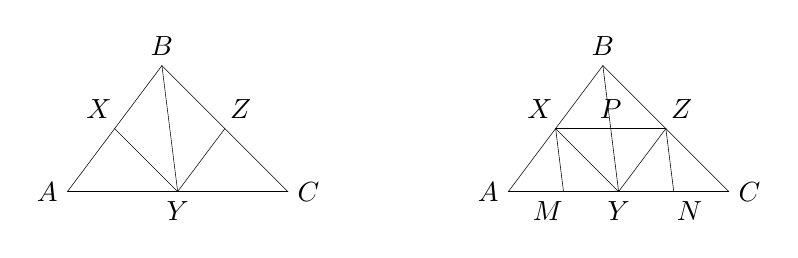
\begin{tikzpicture}[scale=0.8]
    \tkzDefPoint(-4.5,0){A}
    \tkzDefPoint(-3,2){B}
    \tkzDefPoint(-1,0){C}
    \tkzDrawSegments(A,B B,C A,C)
    \tkzLabelPoints[left](A)
    \tkzLabelPoints[above](B)
    \tkzLabelPoints[right](C)
    \tkzDefMidPoint(A,B) \tkzGetPoint{X}
    \tkzDefLine[orthogonal=through X](A,B)
    \tkzDefMidPoint(A,C) \tkzGetPoint{Y}
    \tkzDefLine[orthogonal=through Y](A,C)
    \tkzDefMidPoint(B,C) \tkzGetPoint{Z}
    \tkzDefLine[orthogonal=through Z](B,C)
    \tkzDrawSegment(B,Y)
    \tkzDrawSegment(Y,X)
    \tkzDrawSegment(Y,Z)
    \tkzLabelPoints[above, xshift=-2mm](X)
    \tkzLabelPoints[above, xshift=2mm](Z)
    \tkzLabelPoints[below,yshift=0pt](Y)

    \tkzDefPoint(2.5,0){A}
    \tkzDefPoint(4,2){B}
    \tkzDefPoint(6,0){C}
    \tkzDrawSegments(A,B B,C A,C)
    \tkzLabelPoints[left](A)
    \tkzLabelPoints[above](B)
    \tkzLabelPoints[right](C)
    \tkzDefMidPoint(A,B) \tkzGetPoint{X}
    \tkzDefLine[orthogonal=through X](A,B)
    \tkzDefMidPoint(A,C) \tkzGetPoint{Y}
    \tkzDefLine[orthogonal=through Y](A,C)
    \tkzDefMidPoint(B,C) \tkzGetPoint{Z}
    \tkzDefLine[orthogonal=through Z](B,C)
    \tkzDrawSegment(B,Y)
    \tkzDrawSegment(Y,X)
    \tkzDrawSegment(Y,Z)
    \tkzLabelPoints[above, xshift=-2mm](X)
    \tkzLabelPoints[above, xshift=2mm](Z)
    \tkzLabelPoints[below,yshift=0pt](Y)

    \tkzDefMidPoint(B,Y) \tkzGetPoint{P}
      \tkzDefLine[orthogonal=through P](B,Y)
      \tkzDefMidPoint(A,Y) \tkzGetPoint{M}
      \tkzDefLine[orthogonal=through M](A,Y)
      \tkzDefMidPoint(C,Y) \tkzGetPoint{N}
      \tkzDefLine[orthogonal=through N](C,Y)
      \tkzDrawSegment(X,P)
      \tkzDrawSegment(Z,P)
      \tkzDrawSegment(X,M)
      \tkzDrawSegment(Z,N)
      \tkzLabelPoints[below, xshift=-2mm](M)
    \tkzLabelPoints[below, xshift=2mm](N)
    \tkzLabelPoints[above,yshift=0pt](P)
    \end{tikzpicture}
    \caption{Illustration of newest vertex bisection for Claim 1(left); Claim 2(right)}
    \end{figure}



    Notice that in Stage 3, we see triangles in congruency class 1 again, so we can tell further applying the newest vertex bisection refinement will lead to the same process as what we have for Stage 1. Similarly, further applying the newest vertex bisection refinement over triangles in congruency class 4, 2 and 3 are already explored in Stage 3 and 4. Therefore, we actually obtain 4 congruency classes only.
    \end{proof}
    This means that we never have triangles degenerating when applying the newest vertex bisection refinement, because the number of congruence classes is four, which is finite, and by theorem proved in 3.1, we see that the newest vertex bisection refinement strategy is stable.

    As we explain in section 3, a good refinement strategy should preserve both stability and consistency. Before we take a look at consistency, let's first introduce dependency graph.

    \subsection{Compatible Divisibility and Consistency}
    \begin{definition*}
      Let G = (V, E) be a directed graph, where V represents triangles, and $(V_1, V_2)\in E$ if the refinement edge of $v_1$ neighbors at $v_2$, and then we call G a dependency graph.
      \begin{align*}
      V &= \{Triangles\}\\
      E &= \{(V_1, V_2)\in V\times V | \text{The refinement edge of $V_1$ neighbors $V_2$}\}
      \end{align*}
    \end{definition*}
    Note that $V$ and $E$ in this definition are quite different from general geometry, and all nodes of one dependency graph have at most one outgoing edge (See Figure 9).[Multiple V's, graph? need proof???]
    \begin{figure}[h!]
    \centering
    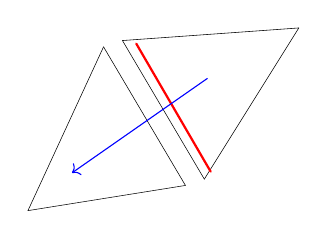
\begin{tikzpicture}[scale=0.8]
    \tkzDefPoint(0.5,0.1){A}
    \tkzDefPoint(3,0.5){B}
    \tkzDefPoint(1.7,2.7){C}
    \tkzDrawSegments(A,B B,C A,C)

    \tkzDefPoint(2,2.8){A'}
    \tkzDefPoint(3.3,0.6){B'}
    \tkzDefPoint(4.8,3){C'}
    \tkzDrawSegments(A',B' B',C' A',C')

    \tkzDefPoint(2.22,2.75){X}
    \tkzDefPoint(3.4,0.72){Y}
    \tkzDrawSegment[thick, color=red](X, Y)
    \draw [blue,  ->   ] (3.35,2.2) -- (1.2,0.7);
    \end{tikzpicture}
    \caption{Illustration of outgoing arrow in dependency graph}
    \label{Figure 9}
    \end{figure}


    \begin{definition*}
      A triangle is called compatibly divisible if either
      \begin{itemize}
        \item[a. ] it has no outgoing edge in G
        \item[b. ] it is part of a cycle in G whose size is 2.
      \end{itemize}
    \end{definition*}
    \begin{figure}[h!]
    \centering
    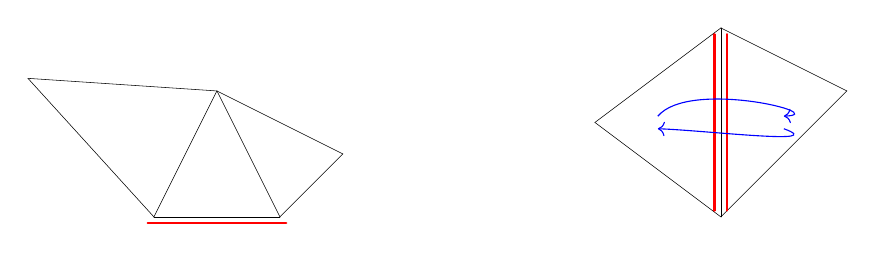
\begin{tikzpicture}[scale=0.8]
    \tkzDefPoint(-4,0){A}
    \tkzDefPoint(-3,2){B}
    \tkzDefPoint(-2,0){C}
    \tkzDrawSegments(A,B B,C A,C)
    \tkzDefPoint(-6,2.2){D}
    \tkzDrawSegments(A,D B,D)
    \tkzDefPoint(-1,1){E}
    \tkzDrawSegments(C,E B,E)
    %\tkzDefPoint(-5,0.5){F}
    %\tkzDrawSegments(A,F)
    %\tkzDefPoint(-1.5,0){G}
    %\tkzDrawSegments(C,G)
    \tkzDefPoint(-4.1,-0.1){X}
    \tkzDefPoint(-1.9,-0.1){Y}
    \tkzDrawSegment[thick, color=red](X, Y)

    \tkzDefPoint(3,1.5){A'}
    \tkzDefPoint(5,0){B'}
    \tkzDefPoint(5,3){C'}
    \tkzDrawSegments(A',B' B',C' A',C')
    \tkzDefPoint(7,2){D'}
    \tkzDrawSegments(B',D' C',D')
    \tkzDefPoint(4.9,0.1){X'}
    \tkzDefPoint(4.9,2.9){Y'}
    \tkzDefPoint(5.1,0.1){M'}
    \tkzDefPoint(5.1,2.9){N'}
    \tkzDrawSegment[thick, color=red](X', Y')
    \tkzDrawSegment[thick, color=red](M', N')

    \draw [->, blue] (4, 1.6) to [out=50,in=2] (6, 1.6);
    \draw [->, blue] (6, 1.4) to [out=-20,in=-2] (4, 1.4);
    \end{tikzpicture}
    \caption{Compatibly divisible triangles: case a(left); case b(right)}
    \label{Figure 10}
    \end{figure}
    Triangles of case b in Figure above are called mates as they share same refinement edge in 2-cycle.

    \noindent
    {Compatible divisibility in Dependency Graph}
    \begin{figure}[h!]
    \centering
    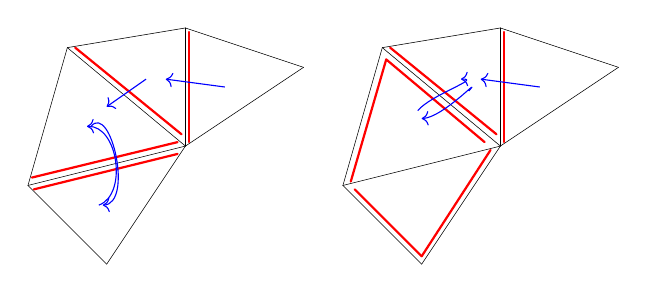
\begin{tikzpicture}[scale=0.5]
    \tkzDefPoint(2,2.5){A}
    \tkzDefPoint(5,0){B}
    \tkzDefPoint(5,3){C}
    \tkzDrawSegments(A,B B,C A,C)
    \tkzDefPoint(8,2){D}
    \tkzDrawSegments(B,D C,D)
    \tkzDefPoint(1,-1){E}
    \tkzDrawSegments(A,E B,E)
    \tkzDefPoint(3,-3){F}
    \tkzDrawSegments(E,F B,F)

    \tkzDefPoint(5.1,2.9){X}
    \tkzDefPoint(5.1,0.1){Y}
    \tkzDrawSegment[thick, color=red](X, Y)
    \tkzDefPoint(2.2, 2.5){X'}
    \tkzDefPoint(4.9, 0.3){Y'}
    \tkzDrawSegment[thick, color=red](X', Y')
    \tkzDefPoint(1.1,-0.8){M}
    \tkzDefPoint(4.8,0.1){N}
    \tkzDrawSegment[thick, color=red](M, N)
    \tkzDefPoint(1.15,-1.1){M'}
    \tkzDefPoint(4.8,-0.2){N'}
    \tkzDrawSegment[thick, color=red](M', N')

    \draw [blue,  ->   ] (6,1.5) -- (4.5,1.7);
    \draw [blue,  ->   ] (4,1.7) -- (3,1);
    \draw [->, blue] (2.6, 0.5) to [out=50,in=2] (2.9, -1.5);
    \draw [->, blue] (2.8, -1.5) to [in=2,out=20] (2.5, 0.5);


    \tkzDefPoint(10,2.5){A}
    \tkzDefPoint(13,0){B}
    \tkzDefPoint(13,3){C}
    \tkzDrawSegments(A,B B,C A,C)
    \tkzDefPoint(16,2){D}
    \tkzDrawSegments(B,D C,D)
    \tkzDefPoint(9,-1){E}
    \tkzDrawSegments(A,E B,E)
    \tkzDefPoint(11,-3){F}
    \tkzDrawSegments(E,F B,F)

    \tkzDefPoint(13.1,2.9){X}
    \tkzDefPoint(13.1,0.1){Y}
    \tkzDrawSegment[thick, color=red](X, Y)
    \tkzDefPoint(10.2, 2.5){X'}
    \tkzDefPoint(12.9, 0.3){Y'}
    \tkzDrawSegment[thick, color=red](X', Y')

    \tkzDefPoint(10.1,2.2){M}
    \tkzDefPoint(12.6,0.1){N}
    \tkzDrawSegment[thick, color=red](M, N)
    \tkzDefPoint(9.2,-0.9){M'}
    \tkzDefPoint(10.1,2.2){N'}
    \tkzDrawSegment[thick, color=red](M', N')

    \tkzDefPoint(9.3,-1.1){K}
    \tkzDefPoint(11,-2.8){L}
    \tkzDrawSegment[thick, color=red](K, L)
    \tkzDefPoint(12.75,-0.1){K'}
    \tkzDefPoint(11,-2.8){L'}
    \tkzDrawSegment[thick, color=red](K', L')

    \draw [blue,  ->   ] (14,1.5) -- (12.5,1.7);
    \draw [blue,  ->   ] (12.2,1.4) to [out=50,in=2] (11,0.7);
    \draw [blue,  ->   ] (10.9,0.9) to [out=50,in=2] (12,1.7);
    %\draw [->, blue] (10.6, 0.5) to [out=50,in=2] (10.9, -1.5);
    %\draw [->, blue] (10.8, -1.5) to [in=2,out=20] (10.5, 0.5);
    \end{tikzpicture}
    \caption{Compatible divisibility in Dependency Graph}
    \end{figure}
    In Figure 11, we see a compatibility chain in a triangulation. When performing the newest vertex bisection on the right most triangle, we need to bisect its left neighboring triangle first. We obtain a recursion here since we need to bisect the triangle which our current target triangle depends on. If we successfully reached the base case, either on boundary or a cycle of size 2, we can then bisect back in an order like stack. In the example displayed in Figure 11, a base case is reached by bisecting the left most two triangles. However, a base case is not always promised. In other word, it is not guaranteed that we can always achieve either bisection on the boundary or a cycle of size 2. One example is displayed in Figure 12, and this failed in applying the newest vertex bisection, because smaller triangles are dependent on each other. That is, its dependency graph is a cycle instead of a forest, i.e. collection of trees.

    \begin{figure}[h!]
    \centering
    %\newdimen\R
    %\R=0.8cm
    \usetikzlibrary{calc}
\tikzset{
parallel segment/.style={
   segment distance/.store in=\segDistance,
   segment pos/.store in=\segPos,
   segment length/.store in=\segLength,
   to path={
   ($(\tikztostart)!\segPos!(\tikztotarget)!\segLength/2!(\tikztostart)!\segDistance!90:(\tikztotarget)$) -- 
   ($(\tikztostart)!\segPos!(\tikztotarget)!\segLength/2!(\tikztotarget)!\segDistance!-90:(\tikztostart)$)  \tikztonodes
   }, 
   % Default values
   segment pos=.5,
   segment length=18ex,
   segment distance=1mm,
},
}
    \begin{tikzpicture}[scale=0.8]
    %\draw (0:\R) \foreach \x in {60,120,...,359} {
    %            -- (\x:\R)
     %}-- cycle (90:\R) node[above] {$n=6$} ;

    \coordinate (A) at (0,0);
    \coordinate (B) at (3,0);
    \tkzDefEquilateral(B,A)\tkzGetPoint{C};
    \tkzDrawPolygon(A,B,C);
    \tkzDefEquilateral(C,A)\tkzGetPoint{D};
    \tkzDrawPolygon(A,C,D);
    \tkzDefEquilateral(C,D)\tkzGetPoint{E};
    \tkzDrawPolygon(E,C,D);
    \tkzDefEquilateral(C,E)\tkzGetPoint{F};
    \tkzDrawPolygon(C,E,F);
    \tkzDefEquilateral(C,F)\tkzGetPoint{G};
    \tkzDrawPolygon(C,F,G);
    \tkzDefEquilateral(C,G)\tkzGetPoint{H};
    \tkzDrawPolygon(C,G,H);

    \draw[red] (A) to[parallel segment] (C);
    \draw[red] (D) to[parallel segment] (C);
    \draw[red] (E) to[parallel segment] (C);
    \draw[red] (F) to[parallel segment] (C);
    \draw[red] (G) to[parallel segment] (C);
    \draw[red] (B) to[parallel segment] (C);
    \end{tikzpicture}
    \caption{Failure of applying newest vertex bisection}
    \end{figure}


    \begin{lemma*}
    If the newest vertex bisection is only performed on 
    \begin{itemize}
        \item[a. ] triangles isolated in the dependency graph
        \item[b. ] pairs of mates
      \end{itemize}
    then the refinement is stable and the triangulations will be consistent.
    \end{lemma*}
    \begin{proof}
    We already proved stability in general in 2 dimension, and this applies here as well under a more strict condition. The consistency is obvious in compatibility divisible triangles.
    \end{proof}

  \section{Discussion and Outlook}
    %\subsection{Discussion}
Changing focus from 2 dimension to 3 dimension for mesh refinement, we confront with more challenges to preserve stability and consistency. In this section, we take a brief look at difficulties in applications of uniform refinement strategy and newest vertex bisection in 3 dimension.

\subsection{Uniform Refinement in 3D}
graphs :-)\\
coordinate proof for two consistency class
\subsection{Newest Vertex Bisection in 3D}
initial refinement edge (Douglas)\\
Possible other bisection algorithm and comparison:



  \newpage
  %\bibliographystyle{abbrvnat}
  \bibliographystyle{plain}
  %\bibliographystyle{apa}
  \bibliography{Bib}
    
  %\subsection{}
\end{document}